%This is the first chapter of the dissertation

%The following command starts your chapter. If you want different titles used in your ToC and at the top of the page throughout the chapter, you can specify those values here. Since Columbia doesn't want extra information in the headers and footers, the "Top of Page Title" value won't actually appear.

\chapter[Results][Top of Page Title]{Title of Chapter 1}

This chapter presents the results of the analysis presented in the previous chapter.
We present the full set of signal region distributions after applying the $\mu$ factors derived from the fitting procedure.
We also present the systematic uncertainties in each signal region properly accounting for the correlations of the uncertainties.
As no excess is observed, we show exclusion limits in the sparticle-\lsp plane based on the results of the model-dependent fits and present the model-independent limits.

\section{Signal region distributions}

In \ref{fig:srs_scale,fig:srg_scale,fig:src_scale}, we can see the unblinded distributions of the last scale cut used for each signal region.
These distributions include the $\mu$ scale factors as well as the systematic uncertainties after the fitting procedure.
Each plot shows the distribution from a signal model which is targetted by the given signal region.

These distributions have all cuts applied except for the cut on this scale variable, which allows us to see the additional discrimination provided by the given variable.
Since signal regions with the same numeral have identical cuts on all cuts other than the main scale variable, we show (a) and (b) on the same figure.
The left-most (right-most) arrow shown is the location of the a (b) cut applied in the analysis.
We call these plot \textit{$N-1$} plots, where $N$ refers to the number of cuts applied in the analysis.
The full set of $N-1$ plots in the signal regions for the other variables used in the analysis are shown in \ref{app:n-1_plots}.

A figure showing a summary of the pulls in all of the SRs is shown in \ref{fig:sr_summary}.
This figure shows the integrated data and simulation values above the cut values in the N-1 plots, with the corresponding statistical and systematic uncertainties, for all signal regions simulatneously.
The systematic uncertainties will be discussed in the next section.
From this plot, we can see there is no significant excess of events over the Standard Model background.

This information is also presented in \ref{tab:p0_UL_RJR}.
The table includes the expectations from simulation before applying the $\mu$ scaling factor.
SRG3b shows a small excess, but this is not significant.

In this case, we set both simplified model-dependent limits and model-independent limits on the possible cross-sections from BSM physics.
\begin{figure}[tbph]
\begin{center}
\includegraphics[width=0.45\textwidth]{ATLAS-CONF-2016-078_INT/N-1Plots/AtlasStyle/Preliminary/SR_SRJigsawSRC1_LastCut_SR_minusone}
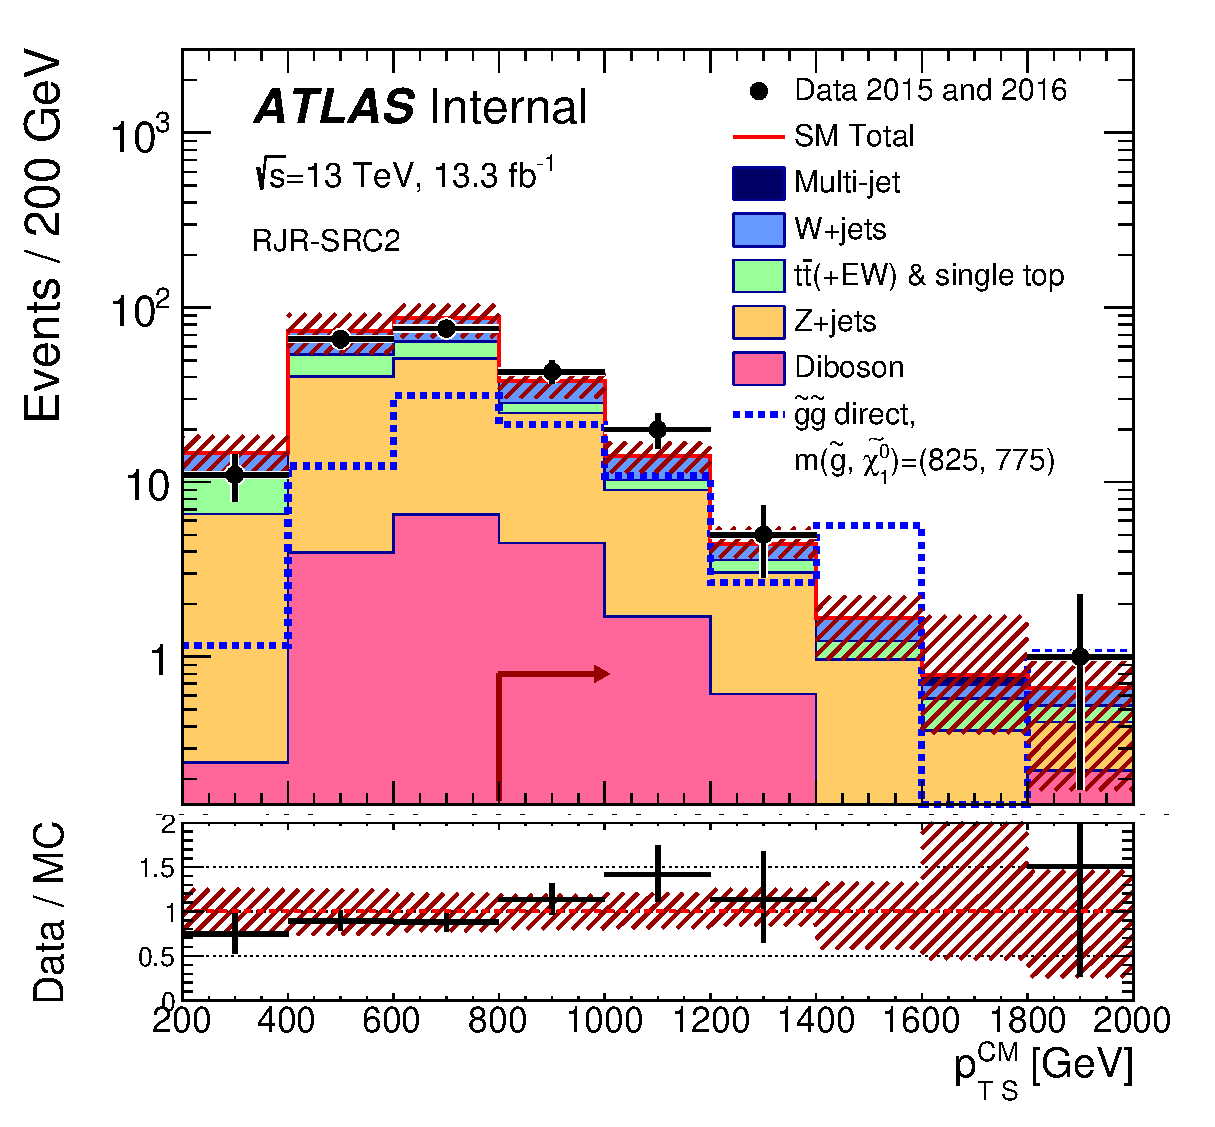
\includegraphics[width=0.45\textwidth]{ATLAS-CONF-2016-078_INT/N-1Plots/AtlasStyle/Preliminary/SR_SRJigsawSRC2_LastCut_SR_minusone}
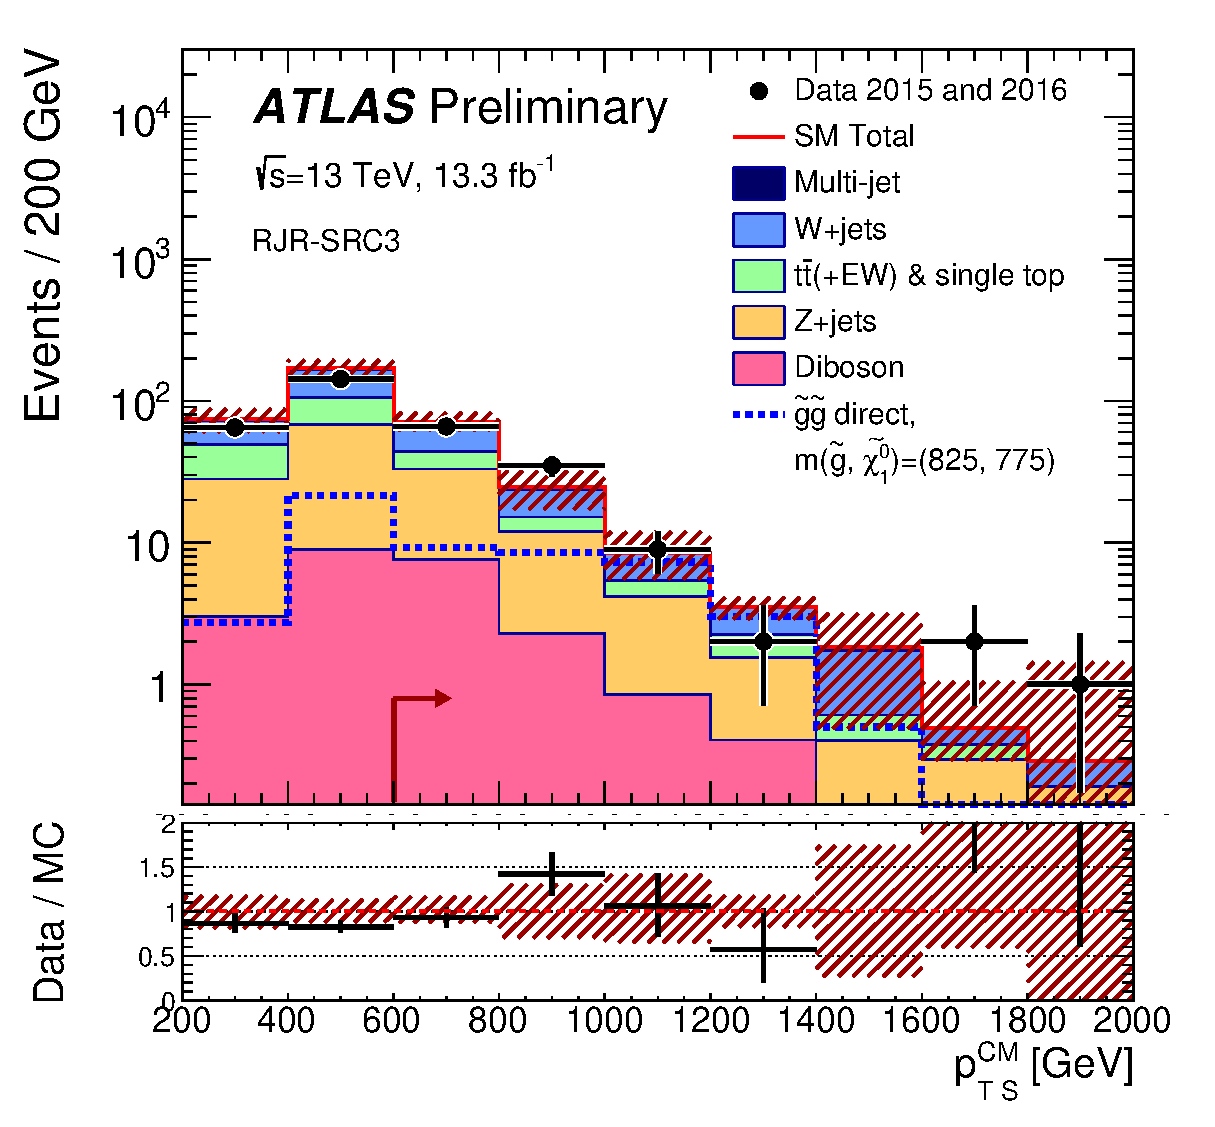
\includegraphics[width=0.45\textwidth]{ATLAS-CONF-2016-078_INT/N-1Plots/AtlasStyle/Preliminary/SR_SRJigsawSRC3_LastCut_SR_minusone}
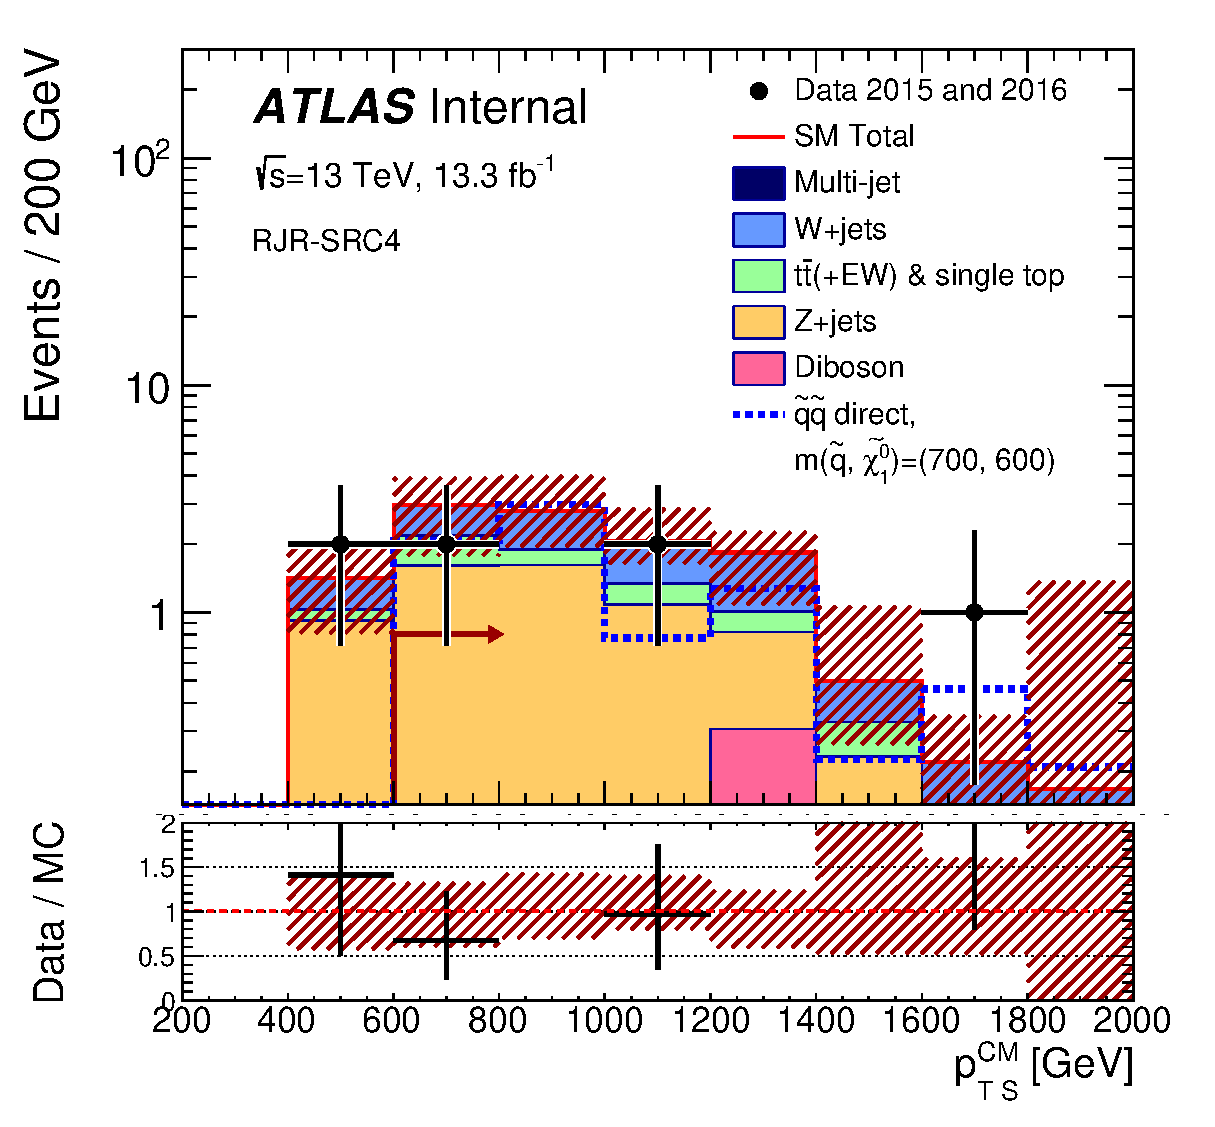
\includegraphics[width=0.45\textwidth]{ATLAS-CONF-2016-078_INT/N-1Plots/AtlasStyle/Preliminary/SR_SRJigsawSRC4_LastCut_SR_minusone}
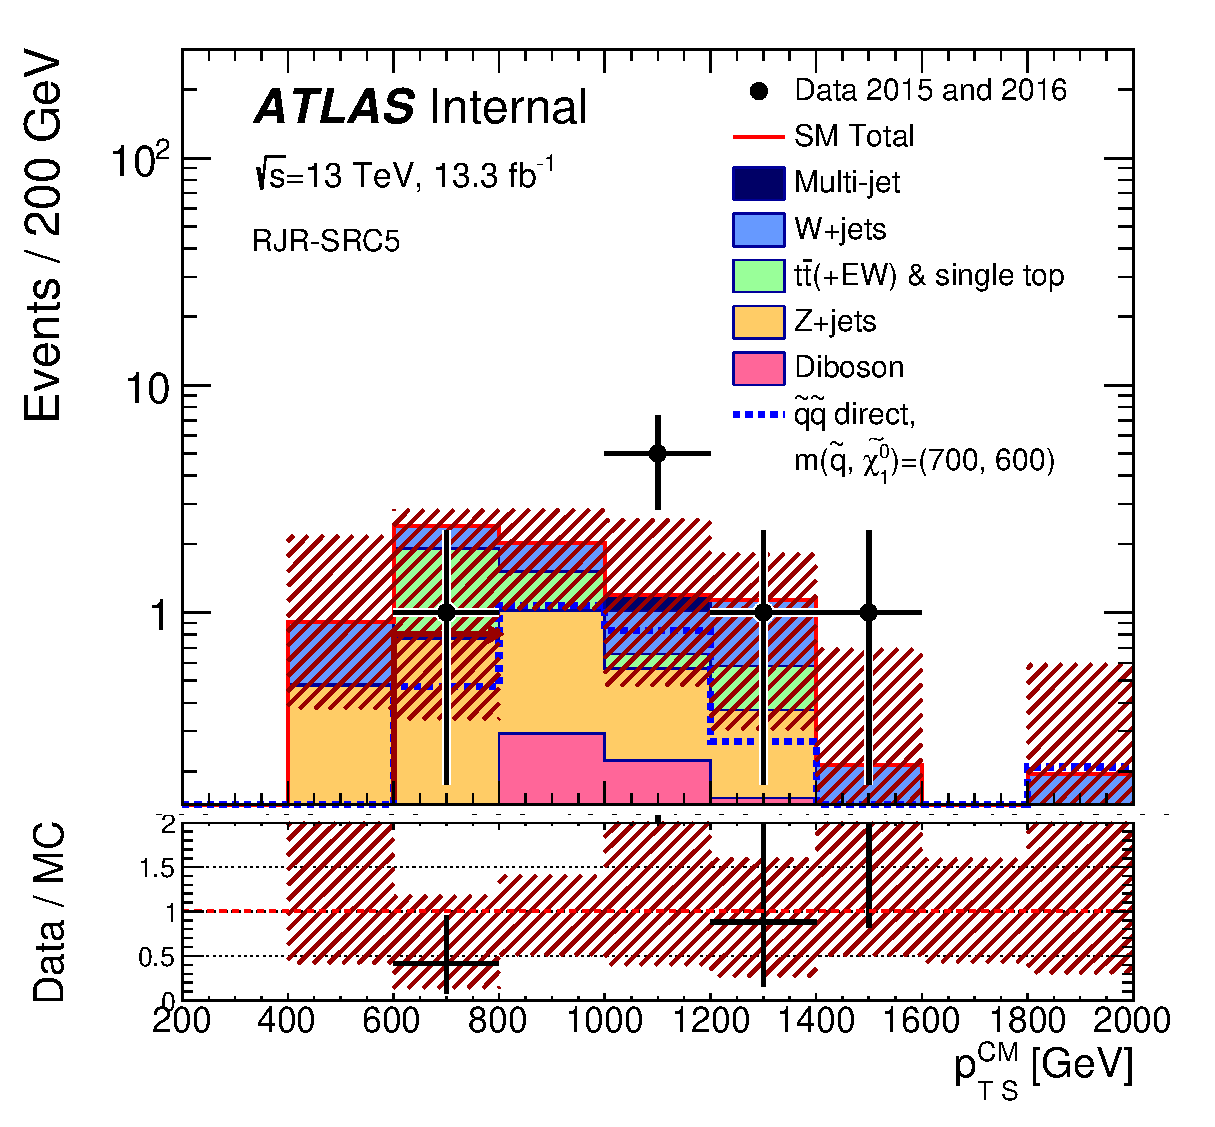
\includegraphics[width=0.45\textwidth]{ATLAS-CONF-2016-078_INT/N-1Plots/AtlasStyle/Preliminary/SR_SRJigsawSRC5_LastCut_SR_minusone}
\end{center}
\caption{}
\label{fig:src_scale}
\end{figure}

\begin{figure}[tbph]
\begin{center}
\includegraphics[width=0.45\textwidth]{ATLAS-CONF-2016-078_INT/N-1Plots/AtlasStyle/Preliminary/SR_SRJigsawSRG1a_LastCut_SR_minusone}
\includegraphics[width=0.45\textwidth]{ATLAS-CONF-2016-078_INT/N-1Plots/AtlasStyle/Preliminary/SR_SRJigsawSRG2a_LastCut_SR_minusone}
\includegraphics[width=0.45\textwidth]{ATLAS-CONF-2016-078_INT/N-1Plots/AtlasStyle/Preliminary/SR_SRJigsawSRG3a_LastCut_SR_minusone}
\end{center}
\caption{}
\label{fig:srg_scale}
\end{figure}

\begin{figure}[tbph]
\begin{center}
\includegraphics[width=0.45\textwidth]{ATLAS-CONF-2016-078_INT/N-1Plots/AtlasStyle/Preliminary/SR_SRJigsawSRS1a_LastCut_SR_minusone}
\includegraphics[width=0.45\textwidth]{ATLAS-CONF-2016-078_INT/N-1Plots/AtlasStyle/Preliminary/SR_SRJigsawSRS2a_LastCut_SR_minusone}
\includegraphics[width=0.45\textwidth]{ATLAS-CONF-2016-078_INT/N-1Plots/AtlasStyle/Preliminary/SR_SRJigsawSRS3a_LastCut_SR_minusone}
\end{center}
\caption{}
\label{fig:srs_scale}
\end{figure}

\begin{figure}[tbph]
\centering
\caption{Summary of the signal region pulls} \label{fig:sr_summary}
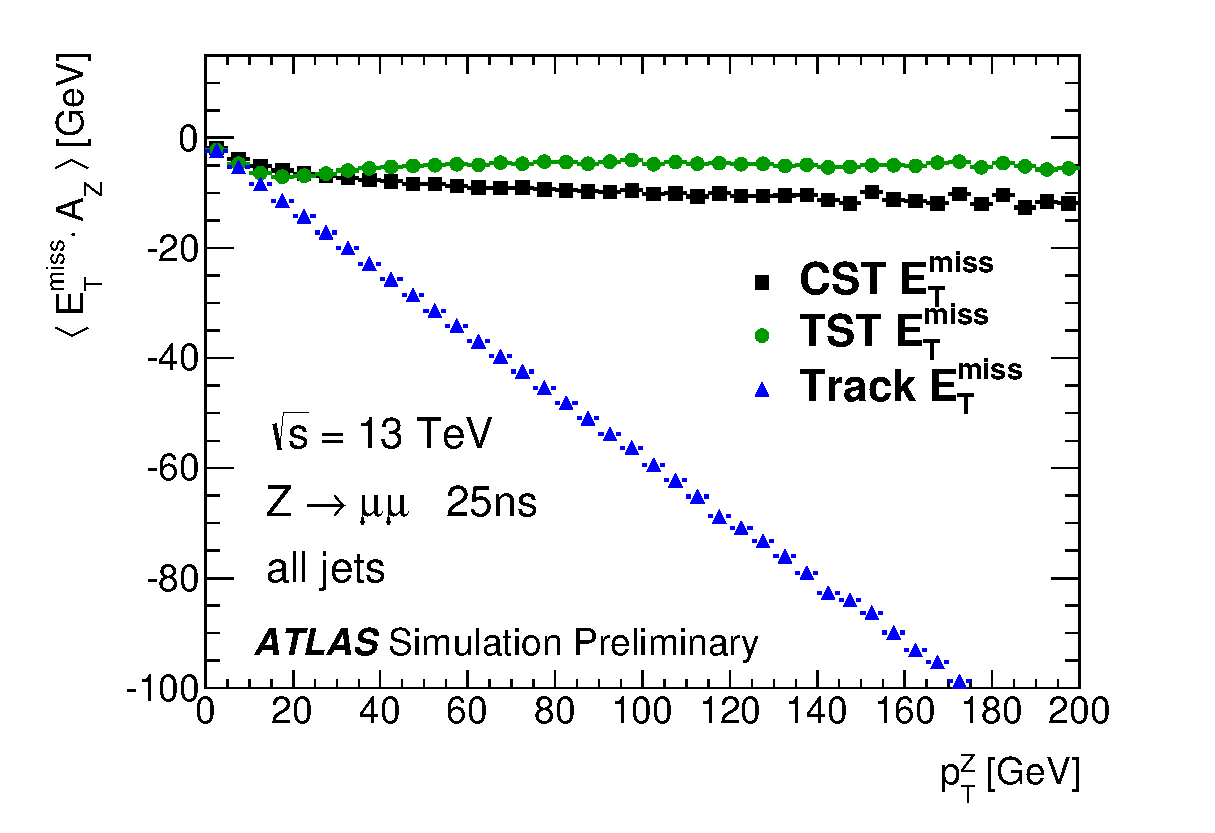
\includegraphics[width=.9\linewidth]{ATLAS-CONF-2016-078/fig_06b}
\end{figure}
\begin{table}[tbph]
\tiny
%\small
\begin{center}
\vspace*{-0.035\textwidth}
\begin{tabular}{|lrrrrrr|}
\hline
Signal Region & \textbf{ RJR-S1a } & \textbf{ RJR-S1b } & \textbf{ RJR-S2a } & \textbf{ RJR-S2b } & \textbf{ RJR-S3a } & \textbf{ RJR-S3b } \\
\hline
\multicolumn{7}{|c|}{MC expected events} \\ \hline
Diboson &  $17$               &  $13$               &  $5.6$               &  $5.1$               &  $4.2$               &  $2.8$               \\
$\mathrm{Z/\gamma^{*}}$+jets &  $231$               &  $163$               &  $63$               &  $48$               &  $36$               &  $24$               \\
W+jets &  $97$               &  $66$               &  $22$               &  $16$               &  $11$               &  $7.8$               \\
$\ttbar$(+EW) + single top &  $15$               &  $10$               &  $2.9$               &  $2.1$               &  $1.7$               &  $1.1$               \\
%%Multi-jet &  $0.93$               &  $0.53$               &  $0.13$               &  $0.00$               &  $0.00$               &  $0.00$               \\
\hline
\multicolumn{7}{|c|}{Fitted background events} \\ \hline
Diboson & $17 \pm 9$ & $13 \pm 7$ & $5.6 \pm 2.8$ & $5.1 \pm 2.6$ & $4.2 \pm 2.1$ & $2.8 \pm 1.4$ \\
$\mathrm{Z/\gamma^{*}}$+jets & $207 \pm 33$ & $146 \pm 23$ & $65 \pm 9$ & $50 \pm 7$ & $37 \pm 5$ & $25.0 \pm 3.5$ \\
W+jets & $95 \pm 9$ & $65 \pm 7$ & $24.1 \pm 2.9$ & $18.3 \pm 2.3$ & $12.8 \pm 2.8$ & $8.7 \pm 2.0$ \\
$\ttbar$(+EW) + single top & $14 \pm 7$ & $9 \pm 5$ & $2.1 \pm 1.7$ & $1.6 \pm 1.3$ & $1.3 \pm 1.0$ & $0.8 \pm 0.7$ \\
Multi-jet &  $0.71_{-0.71}^{+0.71}$               &  $0.41_{-0.41}^{+0.41}$               &  $0.08_{-0.08}^{+0.09}$               & -- & -- & -- \\
\hline
Total Expected MC &  $362$               &  $253$               &  $93$               &  $72$               &  $53$               &  $36$               \\
\hline
Total Fitted bkg & $334 \pm 35$ & $233 \pm 25$ & $96 \pm 10$ & $75 \pm 8$ & $56 \pm 6$ & $37 \pm 4$ \\
\hline
Observed &  $368$                     &  $270$                     &  $99$                     &  $75$                     &  $57$                     &  $36$                     \\
\hline


$\langle\epsilon\mathrm{ \sigma}\rangle_\mathrm{ obs}^{95}$ [fb]   &$7.6$  & $6.5$  & $2.2$  & $1.7$ & $1.6$ & $1.1$ \\
$S_\mathrm{ obs}^{95}$     & $101$ & $86$ & $29$ &  $23$ & $22$ & $15$ \\
$S_\mathrm{ exp}^{95}$     & $ { 78 }^{ +27 }_{ -21 }$ & $ { 61 }^{ +22 }_{ -16 }$ & $ { 28 }^{ +11 }_{ -8 }$ & $ { 23}^{ +9}_{ -7 }$ & $ { 20 }^{ +8 }_{ -6 }$ & $ { 16 }^{ +7 }_{ -5 }$  \\
$p_{0}$ ($\mathrm{Z}$)        & $ 0.20$~$(0.84)$ & $ 0.12$~$(1.17)$ & $ 0.44$~$(0.15)$& $ 0.50$~$(0.00)$ &  $ 0.44$~$(0.14)$ &  $ 0.50$~$(0.00)$ \\
\hline
\end{tabular}

% SRJigsawSRS1a    & $7.61$ &  $101.1$ & $ { 78.3 }^{ +27.0 }_{ -21.1 }$ & $0.00$ & $ 0.20$~$(0.84)$ \\%
% SRJigsawSRS1b    & $6.49$ &  $86.2$ & $ { 60.8 }^{ +22.2 }_{ -16.4 }$ & $0.87$ & $ 0.12$~$(1.17)$ \\%
% SRJigsawSRS2a    & $2.20$ &  $29.3$ & $ { 27.8 }^{ +10.9 }_{ -7.8 }$ & $0.56$ & $ 0.44$~$(0.15)$ \\%
% SRJigsawSRS2b    & $1.72$ &  $22.9$ & $ { 23.4 }^{ +9.4 }_{ -6.5 }$ & $0.47$ & $ 0.50$~$(0.00)$ \\% %% NOTE: capped p-value was nan, wrote 0.5 since nObs < nExp
% SRJigsawSRS3a    & $1.62$ &  $21.5$ & $ { 20.4 }^{ +8.4 }_{ -5.8 }$ & $0.56$ & $ 0.44$~$(0.14)$ \\%
% SRJigsawSRS3b    & $1.14$ &  $15.1$ & $ { 16.0 }^{ +6.7 }_{ -4.5 }$ & $0.44$ & $ 0.49$~$(0.03)$ \\%


%\vspace{0.5cm}
%\end{center}
%\end{table}
\begin{tabular}{|lrrrrrr|}
\hline
Signal Region & \textbf{ RJR-G1a } & \textbf{ RJR-G1b } & \textbf{ RJR-G2a } & \textbf{ RJR-G2b } & \textbf{ RJR-G3a } & \textbf{ RJR-G3b } \\
\hline
\multicolumn{7}{|c|}{MC expected events} \\ \hline
Diboson &  $2.6$               &  $1.6$               &  $2.9$               &  $1.1$               &  $0.62$               &  $0.26$               \\
$\mathrm{Z/\gamma^{*}}$+jets &  $18$               &  $8.8$               &  $13$               &  $4.2$               &  $3.1$               &  $0.83$               \\
W+jets &  $11$               &  $4.7$               &  $7.7$               &  $2.0$               &  $1.9$               &  $0.63$               \\
$\ttbar$(+EW) + single top &  $7.4$               &  $3.1$               &  $4.4$               &  $1.1$               &  $0.34$               &  $0.03$               \\
%%Multi-jet &  $0.27$               &  $0.13$               &  $0.53$               &  $0.40$               &  $0.00$               &  $0.00$               \\
\hline
\multicolumn{7}{|c|}{Fitted background events} \\ \hline
Diboson & $2.6 \pm 1.3$ & $1.6 \pm 0.8$ & $2.9 \pm 1.5$ & $1.1 \pm 0.6$ & $0.6 \pm 0.4$ & $0.26 \pm 0.14$ \\
$\mathrm{Z/\gamma^{*}}$+jets & $21.1 \pm 3.1$ & $10.2 \pm 1.6$ & $14.3 \pm 2.5$ & $4.5 \pm 0.8$ & $3.3 \pm 0.6$ & $0.88 \pm 0.19$ \\
W+jets & $10.8 \pm 1.7$ & $4.6 \pm 1.4$ & $6.7 \pm 1.3$ & $1.7 \pm 0.7$ & $1.6 \pm 0.7$ & $0.55 \pm 0.2$ \\
$\ttbar$(+EW) + single top & $5.4 \pm 1.6$ & $2.3 \pm 0.9$ & $3.4 \pm 1.4$ & $0.8 \pm 0.5$ &  $0.26_{-0.26}^{+0.45}$               &  $0.02_{-0.02}^{+0.26}$               \\
Multi-jet & $0.24 \pm 0.24$ & $0.12 \pm 0.12$ & $0.5 \pm 0.5$ & $0.4 \pm 0.4$ & -- & -- \\
\hline
Total Expected MC &  $39$               &  $18$               &  $29$               &  $8.7$               &  $5.9$               &  $1.7$               \\
\hline
Total Fitted bkg & $40 \pm 4$ & $18.8 \pm 2.5$ & $27.8 \pm 3.4$ & $8.5 \pm 1.4$ & $5.8 \pm 1.1$ & $1.7 \pm 0.4$ \\
\hline
Observed &  $39$                     &  $14$                     &  $30$                     &  $10$                     &  $8$                     &  $4$                     \\
\hline


$\langle\epsilon\mathrm{ \sigma}\rangle_\mathrm{ obs}^{95}$ [fb]   & $1.1$   &  $0.56$  &  $1.1$ & $0.71$ & $0.64$ &  $0.55$ \\
$S_\mathrm{ obs}^{95}$     & $15$ & $7.5$ &$15$ & $9.4$ & $8.5$  &  $7.3$ \\
$S_\mathrm{ exp}^{95}$     & $ { 16 }^{ +7 }_{ -4 }$  & $ { 10 }^{ +5 }_{ -3 }$ & $ { 14 }^{ +6 }_{ -4 }$ & $ { 7.6 }^{ +3.5}_{ -2.0 }$ & $ { 7.0 }^{ +2.5}_{ -2.1 }$  & $ { 4.2 }^{ +1.9 }_{ -0.5 }$\\
$p_{0}$ ($\mathrm{Z}$)        & $ 0.50$~$(0.00)$  & $ 0.50$~$(0.00)$ & $ 0.36$~$(0.35)$ & $ 0.31$~$(0.50)$ & $ 0.21$~$(0.81)$ & $ 0.06$~$(1.55)$ \\
\hline
\end{tabular}


% SRJigsawSRG1a    & $1.13$ &  $15.0$ & $ { 15.7 }^{ +6.7 }_{ -4.4 }$ & $0.45$ & $ 0.50$~$(0.00)$ \\% %% NOTE: capped p-value was nan, wrote 0.5 since nObs < nExp
% SRJigsawSRG1b    & $0.56$ &  $7.5$ & $ { 10.3 }^{ +4.8 }_{ -2.9 }$ & $0.18$ & $ 0.50$~$(0.00)$ \\%
% SRJigsawSRG2a    & $1.14$ &  $15.2$ & $ { 13.6 }^{ +5.8 }_{ -3.9 }$ & $0.63$ & $ 0.36$~$(0.35)$ \\%
% SRJigsawSRG2b    & $0.70$ &  $9.3$ & $ { 7.7 }^{ +4.0 }_{ -2.3 }$ & $0.65$ & $ 0.33$~$(0.44)$ \\%
% SRJigsawSRG3a    & $0.67$ &  $8.9$ & $ { 7.1 }^{ +3.0 }_{ -2.2 }$ & $0.73$ & $ 0.23$~$(0.74)$ \\%
% SRJigsawSRG3b    & $0.56$ &  $7.5$ & $ { 7.0 }^{ +2.7 }_{ -2.0 }$ & $0.62$ & $ 0.18$~$(0.93)$ \\%


%\end{center}
%\end{table}
\begin{tabular}{|lrrrrr|}
\hline
Signal Region & \textbf{ RJR-C1 } & \textbf{ RJR-C2 } & \textbf{ RJR-C3 } & \textbf{ RJR-C4 } & \textbf{ RJR-C5 } \\
\hline
\multicolumn{6}{|c|}{MC expected events} \\ \hline
Diboson &  $1.9$               &  $7.1$               &  $11$               &  $0.54$               &  $0.75$               \\
$\mathrm{Z/\gamma^{*}}$+jets &  $8.8$               &  $36$               &  $46$               &  $5.8$               &  $2.5$               \\
W+jets &  $3.5$               &  $16$               &  $43$               &  $3.8$               &  $2.3$               \\
$\ttbar$(+EW) + single top &  $1.9$               &  $7.2$               &  $20$               &  $1.7$               &  $2.5$               \\
%%Multi-jet &  $0.13$               &  $0.53$               &  $3.05$               &  $0.00$               &  $0.27$               \\
\hline
\multicolumn{6}{|c|}{Fitted background events} \\ \hline
Diboson & $1.9 \pm 1.0$ & $7 \pm 4$ & $11 \pm 6$ & $0.54 \pm 0.29$ & $0.8 \pm 0.5$ \\
$\mathrm{Z/\gamma^{*}}$+jets & $7.7 \pm 1.1$ & $32 \pm 5$ & $40 \pm 6$ & $5.0 \pm 0.8$ & $2.2 \pm 0.4$ \\
W+jets & $3.3 \pm 1.4$ & $14.5 \pm 1.7$ & $40 \pm 5$ & $3.56 \pm 1.0$ & $2.14 \pm 0.35$ \\
$\ttbar$(+EW) + single top & $1.5 \pm 0.6$ & $5.8 \pm 1.8$ & $16 \pm 5$ & $1.4 \pm 0.7$ & $2.0 \pm 1.1$ \\
Multi-jet & $0.09 \pm 0.09$ & $0.4 \pm 0.4$ & $2.1 \pm 2.1$ & -- & $0.18 \pm 0.18$ \\
\hline
Total Expected MC &  $16$               &  $67$               &  $124$               &  $12$               &  $8.3$               \\
\hline
Total Fitted bkg & $14.5 \pm 2.2$ & $59 \pm 6$ & $110 \pm 11$ & $10.5 \pm 1.5$ & $7.3 \pm 1.4$ \\
\hline
Observed &  $14$                     &  $69$                     &  $115$                     &  $5$                     &  $8$                     \\
\hline


$\langle\epsilon\mathrm{ \sigma}\rangle_\mathrm{ obs}^{95}$ [fb]   &$0.76$   & $2.2$ & $2.5$  & $0.35$ & $0.61$  \\
$S_\mathrm{ obs}^{95}$     & $10$ & $29$ &  $34$  & $4.7$ & $8.1$ \\
$S_\mathrm{ exp}^{95}$     & $ { 11 }^{ +5 }_{ -3 }$ &  $ { 21 }^{ +9 }_{ -6 }$ & $ { 30 }^{ +12 }_{ -8 }$ & $ { 8.1 }^{ +3.0 }_{ -2.3 }$ & $ { 7.4 }^{ +2.9 }_{ -1.8 }$ \\
$p_{0}$ ($\mathrm{Z}$)        & $ 0.50$~$(0.00)$  & $ 0.18$~$(0.92)$ & $ 0.37$~$(0.32)$ & $ 0.50$~$(0.00)$  & $ 0.39$~$(0.30)$ \\
\hline
\end{tabular}

% SRJigsawSRC1    & $0.76$ &  $10.1$ & $ { 10.6 }^{ +4.6 }_{ -3.1 }$ & $0.46$ & $ 0.50$~$(0.00)$ \\% %% NOTE: capped p-value was nan, wrote 0.5 since nObs < nExp
% SRJigsawSRC2    & $2.15$ &  $28.6$ & $ { 21.1 }^{ +8.7 }_{ -6.0 }$ & $0.81$ & $ 0.18$~$(0.92)$ \\%
% SRJigsawSRC3    & $2.52$ &  $33.5$ & $ { 30.2 }^{ +11.7 }_{ -8.4 }$ & $0.62$ & $ 0.37$~$(0.32)$ \\%
% SRJigsawSRC4    & $0.36$ &  $4.8$ & $ { 7.7 }^{ +4.0 }_{ -2.3 }$ & $0.06$ & $ 0.48$~$(0.06)$ \\%
% SRJigsawSRC5    & $0.61$ &  $8.1$ & $ { 7.5 }^{ +3.6 }_{ -2.4 }$ & $0.59$ & $ 0.41$~$(0.23)$ \\%

\vspace*{-0.01\textheight}\caption[p0 and UL]{Numbers of events observed in the signal regions used in the RJR-based analysis compared with background expectations obtained from the fits described in the text.
Empty cells (indicated by a `-') correspond to estimates lower than $0.01$.
The p-values ($p_{0}$) give the probabilities of the observations being consistent with the estimated backgrounds.
For an observed number of events lower than expected, the p-value is truncated at 0.5. Between parentheses, $p$-values are also given as the number of equivalent Gaussian standard deviations (Z).
Also shown are 95\% CL upper limits on the visible cross-section ($\langle\epsilon\sigma\rangle_\mathrm{ obs}^{95}$),
the visible number of signal events ($S_\mathrm{ obs}^{95}$ ) and the number of signal events ($S_\mathrm{ exp}^{95}$)
given the expected number of background events (and $\pm 1\sigma$ excursions of the expectation).
\label{tab:p0_UL_RJR}}
\end{center}
\end{table}


\section{Fitting procedure checks and systematic uncertainties}

This section


\section{Exclusion plots}

\begin{figure}[tbph]
\centering
\caption{Exclus.}
\label{fig:srs_scale}
\end{figure}
